\chapter{Arquitetura}

\section{Interação entre as partes}
Um utilizador apenas interage com um \textit{broker}. O \textit{broker} comunica-se com o utilizador e com o servidor de armazenamento. O servidor de armazenamento apenas interage com os \textit{brokers}.

\begin{figure}[h]
	\makebox[\textwidth][c]{
		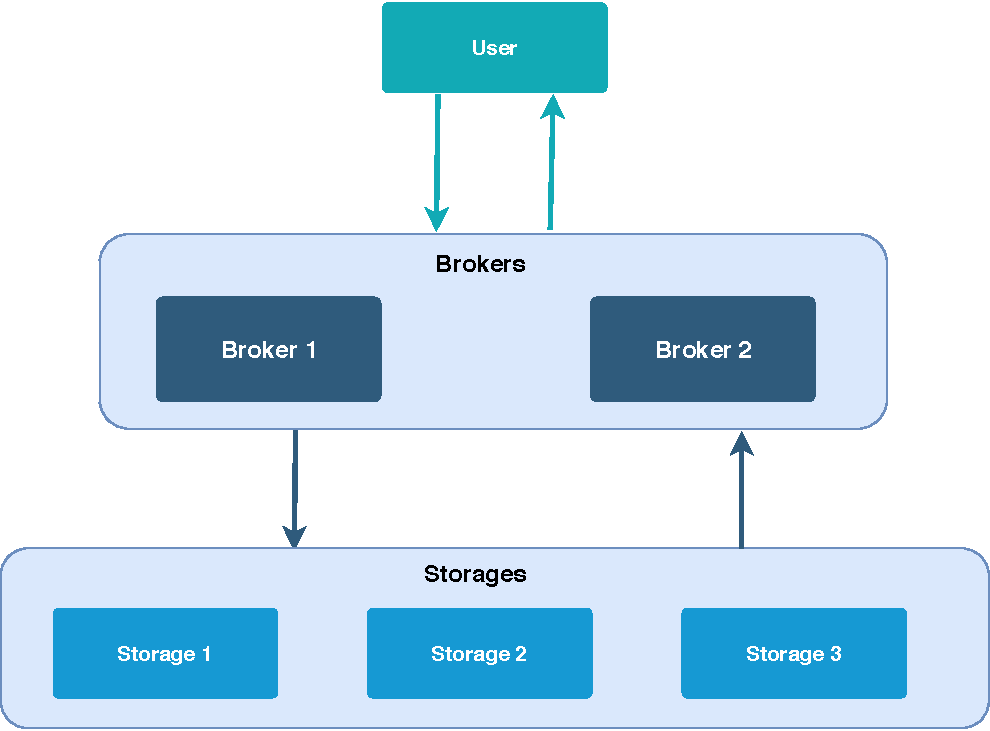
\includegraphics[width=0.8\textwidth]{./figures/architecture.pdf}
	}
	\caption{Arquitetura}
\end{figure}

O utilizador é cliente do \textit{broker}. O \textit{broker} é serviço do utilizador e cliente do servidor de armazenamento. O servidor de armazenamento é serviço do \textit{broker}.

\section{Funcionamento}
Para poder utilizar o sistema, o utilizador deve escolher em qual \textit{broker} pretende-se conectar. Estando este conectado, é possível usufruir das seguintes funcionalidades:
\begin{itemize}
	\item Guardar dados e obter uma chave associada;
	\item Obter os dados através da chave associada;
	\item Eliminar os dados através da chave associada.
\end{itemize}

\subsection{Funcionamento}
Para um utilizador guardar um valor deve primeiro escolher qual o \textit{broker} que deseja conectar-se. Após a escolha do \textit{broker} o utilizador pode inserir um valor e guardá-lo. Ao guardar o valor, a aplicação cliente interage com o \textit{broker} e este, através de um algoritmo de seleção, irá escolher qual o servidor de armazenamento com menor carga. Após guardar o valor, o \textit{broker} gera um chave e envia à aplicação cliente. A aplicação cliente com essa chave pode obter novamente o valor ou apagar dos servidores de armazenamento.

\section{Escalabilidade}
O sistema é escalável horizontalmente. Desta forma, se um dos \textit{brokers} ou servidores de armazenamento ficar sobrecarregado, é possível adicionar mais \textit{brokers} e/ou servidores de armazenamento. Os \textit{brokers} já existentes terão de ser reiniciados para reconhecer os novos servidores de armazenamento.